%%%%%%%%%%%%%%%%%%%%%%%%%%%%%%%%%%%%%%%%%%%%%%%%%%%%%%%%%%%%%%%%%%%%%%%%%%%
%% This file is part of the book
%%
%% Algorithmic Graph Theory
%% http://code.google.com/p/graph-theory-algorithms-book/
%%
%% Copyright (C) 2009, 2010 Minh Van Nguyen <nguyenminh2@gmail.com>
%%
%% See the file COPYING for copying conditions.
%%%%%%%%%%%%%%%%%%%%%%%%%%%%%%%%%%%%%%%%%%%%%%%%%%%%%%%%%%%%%%%%%%%%%%%%%%%

%% graph G
\subfigure[$G$]{
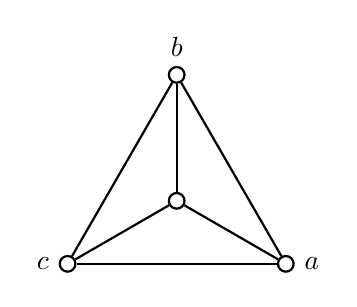
\begin{tikzpicture}
[nodedecorate/.style={shape=circle,inner sep=2pt,draw,thick},%
  linedecorate/.style={-,thick}, scale=1.6]
%% nodes or vertices
\foreach \nodename/\x/\y in {a/0.8660/-0.5, b/0/1, c/-0.8660/-0.5,
  d/0/0}
{
  \node (\nodename) at (\x,\y) [nodedecorate] {};
}
\foreach \nodename/\direction/\navigate in {a/right/east, b/above/north,
  c/left/west}
{
  \node [\direction] at (\nodename.\navigate) {$\nodename$};
}
%% edges or lines
\path
\foreach \startnode/\endnode in {a/b, a/c, a/d, b/c, b/d, c/d} {
  (\startnode) edge[linedecorate] node {} (\endnode)
};
\end{tikzpicture}
}
%%
%% edge deletion subgraph G - {ac}
\subfigure[$G - \{ac\}$]{
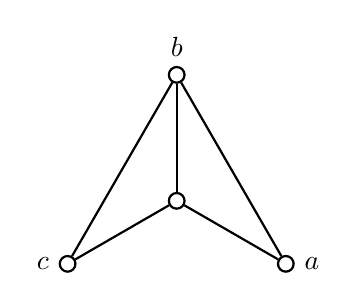
\begin{tikzpicture}
[nodedecorate/.style={shape=circle,inner sep=2pt,draw,thick},%
  linedecorate/.style={-,thick}, scale=1.6]
%% nodes or vertices
\foreach \nodename/\x/\y in {a/0.8660/-0.5, b/0/1, c/-0.8660/-0.5,
  d/0/0}
{
  \node (\nodename) at (\x,\y) [nodedecorate] {};
}
\foreach \nodename/\direction/\navigate in {a/right/east, b/above/north,
  c/left/west}
{
  \node [\direction] at (\nodename.\navigate) {$\nodename$};
}
%% edges or lines
\path
\foreach \startnode/\endnode in {a/b, a/d, b/c, b/d, c/d} {
  (\startnode) edge[linedecorate] node {} (\endnode)
};
\end{tikzpicture}
}
%%
%% edge deletion subgraph G - {ab, ac, bc}
\subfigure[$G - \{ab, ac, bc\}$]{
\label{fig:introduction:skeleton_subgraph_via_edge_deletion}
\begin{tikzpicture}
[nodedecorate/.style={shape=circle,inner sep=2pt,draw,thick},%
  linedecorate/.style={-,thick}, scale=1.6]
%% nodes or vertices
\foreach \nodename/\x/\y in {a/0.8660/-0.5, b/0/1, c/-0.8660/-0.5,
  d/0/0}
{
  \node (\nodename) at (\x,\y) [nodedecorate] {};
}
\foreach \nodename/\direction/\navigate in {a/right/east, b/above/north,
  c/left/west}
{
  \node [\direction] at (\nodename.\navigate) {$\nodename$};
}
%% edges or lines
\path
\foreach \startnode/\endnode in {a/d, b/d, c/d} {
  (\startnode) edge[linedecorate] node {} (\endnode)
};
\end{tikzpicture}
}
